\section{Justificación del Proyecto}
El presente proyecto tiene como objetivo la construcción de un backend para un portal de datos sobre la tierra.  Éste proyecto forma parte a su vez del proyecto \textit{Rebuilding IFAD's LandPortal RFQ/2013/016/SC} desarrollado por el grupo de investigación Web Semantics Oviedo\footnote{WESO - http://www.weso.es/} y la empresa {SB Consulting\footnote{SBC4D - http://www.sbc4d.com/} y que cuenta como cliente con el Fondo Internacional para el Desarrollo Agrícola\footnote{IFAD - http://www.ifad.org/}, perteneciente a la Organización de las Naciones Unidas\footnote{ONU - http://www.un.org/es/}.

El backend que se desarrollará en éste proyecto será por tanto utilizado en la renovación del Land Portal\footnote{http://landportal.info/}.

El Land Portal tiene como objetivo convertirse en el sitio líder a la hora de buscar información y recursos sobre todos los temas relacionados con la tierra. Tal y como Tim Davies explica en \citetitle[página 5]{landportal-strategy}:
\begin{quote}
\textit{``La visión del portal es mejorar la gestión de la tierra para beneficiar a aquellos más vulnerables y con menos derechos, a través de la transmisión de información y conocimiento}.''
\end{quote}

Para alcanzar ésta visión, el Land Portal pretende aumentar el número de países, regiones, indicadores y tópicos sobre los que almacena información, además de mejorar la visualización y reutilización de los nuevos datos y los datos ya existentes.

Por todo ello, y con el objetivo de servir como ejemplo en la transparencia de la información, el Land Portal se encuentra en una fase de crecimiento y expansión, pretendiendo convertirse en un portal de datos abiertos y contribuir a un desarrollo ágil y visible públicamente.



\section{Objetivos del proyecto}
\label{objetivos_proyecto}
El principal objetivo que se pretende cumplir en éste proyecto es la construcción de un portal de datos que permita de centralizar, organizar y buscar información relacionada con la gestión y el uso de la tierra que de otra forma estaría fragmentada e inaccesible.\\
Dicha información procede de diversas fuentes de datos pertenecientes a gobiernos, instituciones académicas, organizaciones internacionales y organizaciones no gubernamentales como pueden ser:
\begin{itemize}
\item el Banco Mundial (\textit{WorldBank})
\item la Organización de las Naciones Unidas para la Alimentación y la Agricultura (\textit{FAO})
\item la Organización Mundial de la Salud (\textit{WHO})
\item el Instituto Internacional de Investigación sobre Políticas Alimentarias (\textit{IFPRI})
\item la Organización para la Cooperación y el Desarrollo Económicos (\textit{OECD})
\end{itemize}
Puesto que los datos proceden de fuentes tan diversas, es importante para el portal centralizar y unificar el proceso de inserción de nuevos datos, con el fin de facilitar la colaboración de entidades externas que quieran ver sus datos reflejados en el portal y, al mismo tiempo, asegurar la calidad de los mismos, haciendo que cumplan unos estándares mínimos de calidad.

Un segundo objetivo de gran importancia para este proyecto es fomentar el diálogo, el intercambio de información y la participación de los usuarios de una forma que permita complementar, combinar y enriquecer la información presentada desde las fuentes de datos oficiales. Para ello es importante contar con un lugar en el que los usuarios puedan debatir y compartir información de una forma sencilla.\newline
En relación con el interés por fomentar la participación de los usuarios en el portal también se pretende simplificar el método de acceso al mismo, de forma que se consiga integrar en un único punto el acceso a todas las partes del portal y al registro e inicio de sesión de los usuarios

Por último, y como no puede ser de otra forma en un portal destinado a almacenar y presentar datos sobre las distintas regiones del mundo, es de especial interés establecer un sistema de internacionalización que permita a los usuarios visualizar la información en el idioma que prefieran y, de esta forma democratizar el acceso a toda la información expuesta.

Éstos objetivos se desarrollarán en mayor detalle en el capítulo \ref{chapter04}.



\section{Estudio de la situación actual}
En la actualidad, los portales de datos son una tendencia que se hace cada vez más presente en el entorno de Internet.  Son varios los gobiernos y organizaciones que cuentan con un portal de datos para facilitar el acceso de los ciudadanos a todo tipo de información.

En esta sección se enumerarán algunos portales de datos abiertos que han servido como referente e inspiración a la hora de construir el nuevo Land Portal, al mismo tiempo que se repasarán las referencias y similitudes con cada uno de ellos.

\subsection{Portal de datos del Gobierno de Estados Unidos}
El portal de datos del Gobierno de Estados Unidos \footnote{http://www.data.gov/} es un referente en cuanto a la construcción de éste tipo de portales.  Fue publicado por primera vez en mayo de 2009 y recibió un rediseño completo en el aniversario de su primer año (el 21 de mayo de 2010).  Actualmente es uno de los portales de datos con mayor cantidad de información, puesto que contiene casi 250000 conjuntos de datos.
\begin{figure}[h]
\centering
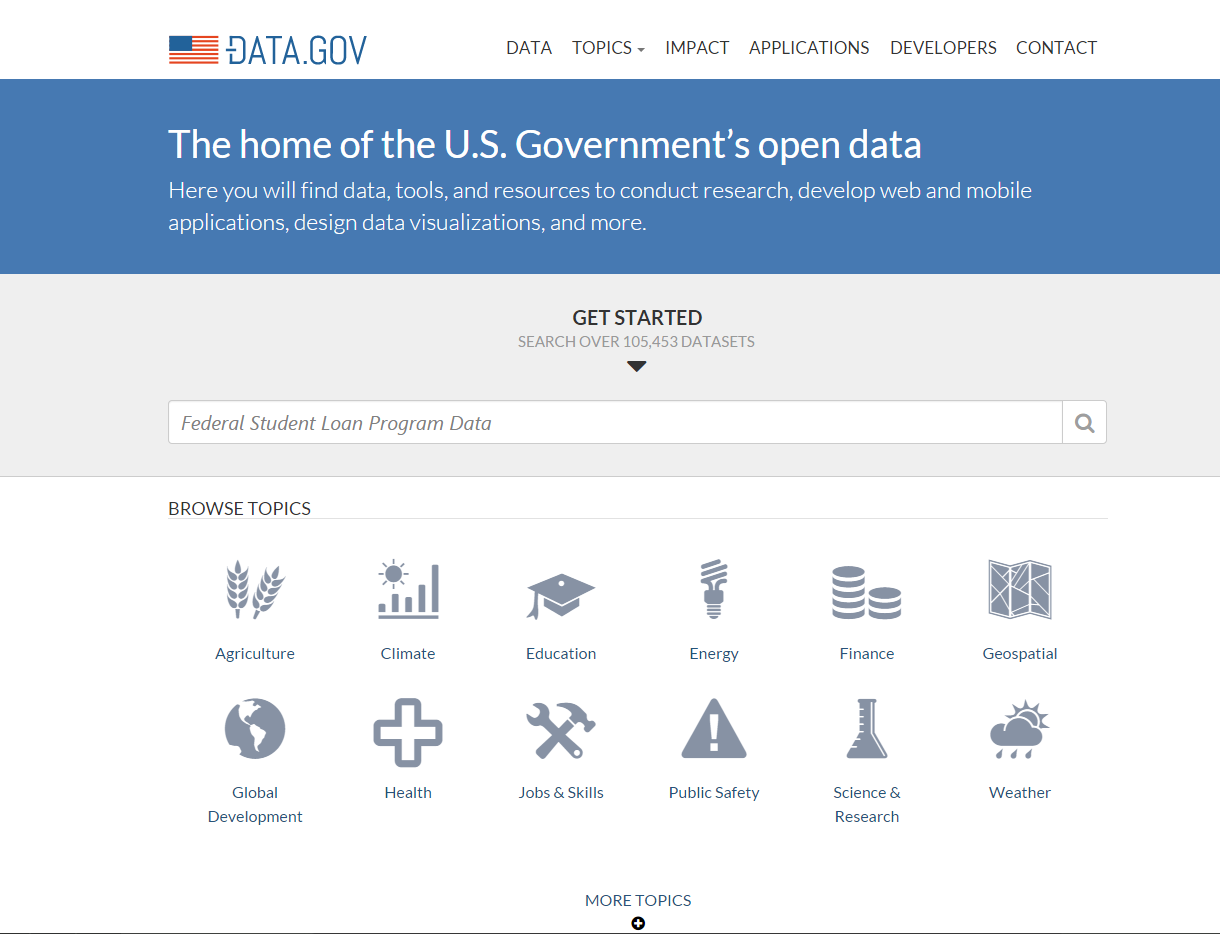
\includegraphics[width=\textwidth]{estado_arte/datagov}
\caption{Página principal del portal de datos del Gobierno de Estados Unidos}
\end{figure}

El portal utiliza CKAN \footnote{http://ckan.org/} para almacenar todos los conjuntos de datos y Drupal\footnote{https://drupal.org/} como gestor de contenidos.

Un apartado en el que el nuevo Land Portal intenta mejorar a éste portal es la visualización de datos. El nuevo Land Portal ofrecerá visualizaciones destinadas a facilitar la interpretación de los datos por parte de los usuarios.

\subsection{Portal de datos del Gobierno Británico}
El portal de datos del Gobierno Británico\footnote{http://data.gov.uk/}, al igual que el portal de datos del Gobierno de Estados Unidos, es también uno de los referentes mundiales en cuanto a portales de datos abiertos.

El portal se hizo público en enero de 2010 y actualmente contiene más de 9000 conjuntos de datos procedentes de varios departamentos del Gobierno.  Todos los conjuntos de datos se encuentran disponibles de forma gratuita para uso privado y comercial siempre que se atribuya su creación al Gobierno Británico.
\begin{figure}[h]
\centering
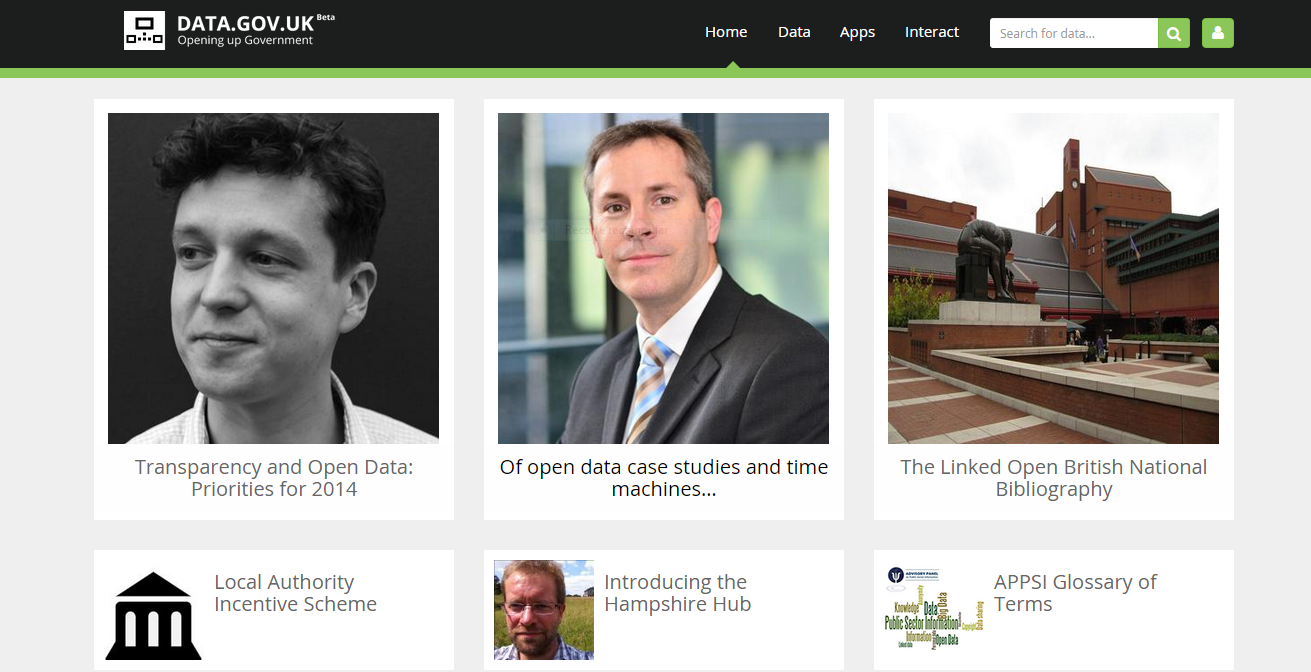
\includegraphics[width=\textwidth]{estado_arte/datagovuk}
\caption{Página principal del portal de datos del Gobierno Británico}
\end{figure}

Al igual que el portal de datos del Gobierno de Estados Unidos, este portal también utiliza CKAN y Drupal como gestor de datos y de contenido respectivamente.  Como se explicará posteriormente en esta misma sección, el nuevo Land Portal también utiliza un sistema similar, debido a su probada estabilidad en sistemas similares.  El aspecto del nuevo Land portal también se ha inspirado en el diseño claro y simple de éste portal.

\subsection{Antiguo Land Portal}
El Land Portal\footnote{http://landportal.info/} pertenece al Fondo Internacional para
el Desarrollo Agrícola, que forma parte de la ONU.  Fue creado en marzo de 2011 y actualmente cuenta con casi 1000 usuarios registrados y un total de 70 organizaciones diferentes. En el año 2012 el portal tuvo unos 70000 visitantes únicos, con cerca de 10000 visitas mensuales\footnote{Ésta información puede consultarse en \cite[página 3]{landportal-strategy}}.
\begin{figure}[h]
\centering
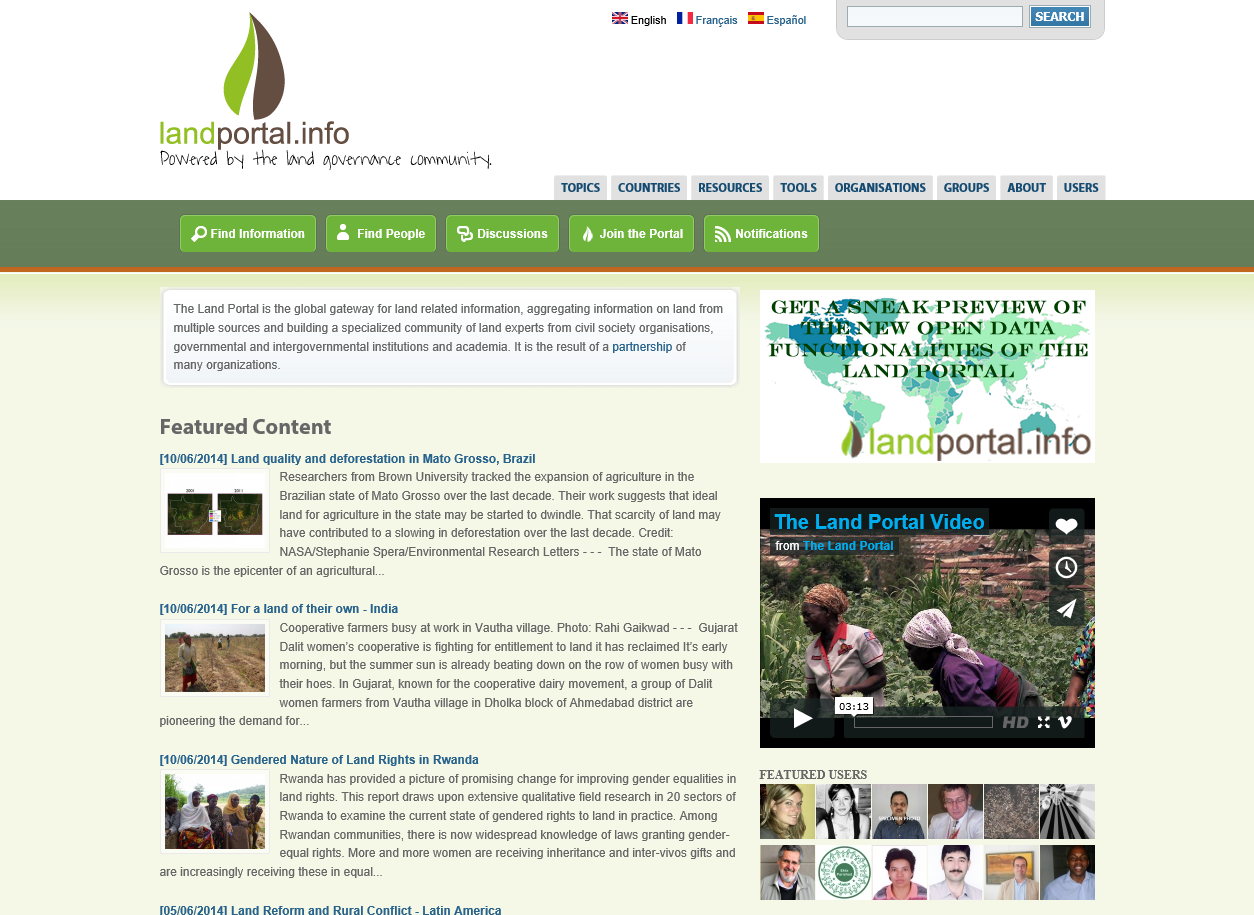
\includegraphics[width=\textwidth]{estado_arte/old_landportal_home}
\caption{Página principal del antiguo Land Portal}
\end{figure}

A pesar de no ser un portal de datos abiertos como tal, el viejo Land Portal ha sido la principal inspiración a la hora de realizar este proyecto. El nuevo portal pretende reunir y mejorar las características de los portales de datos del Gobierno Británico y del Gobierno de Estados Unidos y, al mismo tiempo, mantener el espíritu original de colaboración e intercambio de conocimientos del viejo Land Portal.  Los principales puntos en los que este proyecto pretende mejorar lo ofrecido por el viejo Land Portal son los siguientes:
\begin{itemize}
\item Ofrecer una interfaz más amigable, en línea con la sencillez y vistosidad de los portales de datos del Gobierno Británico y el Gobierno de Estados Unidos.
\item Ofrecer acceso a los conjuntos de datos procedentes de diferentes organizaciones, tanto de forma visual como a través de un API para desarrolladores y un catálogo de datos con capacidad de negociación de contenido.
\item Fomentar la participación de todos los miembros de la comunidad aportando nueva información y debatiendo sobre la ya existente.
\end{itemize}

